\documentclass[11pt]{article}

\usepackage{blindtext}
\usepackage{booktabs}
\usepackage{fullpage}
\usepackage{rotating}   
\usepackage{amsmath}
\usepackage{amssymb}
\usepackage{amsthm}
\usepackage{fancyhdr}
\usepackage{algorithm}
\usepackage{bm}
\usepackage{listings}
\usepackage{graphicx}
\usepackage{caption2}
\usepackage{subfigure}
\usepackage{float}
\usepackage{extpfeil}
\usepackage{color}
\usepackage{indentfirst} 
\usepackage[stable]{footmisc}
\usepackage[usenames,dvipsnames]{xcolor}
\usepackage[noend]{algpseudocode}

\newtheorem{theorem}{Theorem}[section]
\newtheorem{lemma}[theorem]{Lemma}
\newtheorem{corollary}[theorem]{Corollary}
\newtheorem{proposition}[theorem]{Proposition}
\newtheorem{definition}[theorem]{Definition}
\newtheorem{conjecture}[theorem]{Conjecture}
\newtheorem{remark}[subsection]{Remark}

%%
\newcommand\numberthis{\addtocounter{equation}{1}\tag{\theequation}}

%% define new symbols
\def\bx{\bm{x}}
\def\bb{\bm{b}}
\def\ba{\bm{a}}
\def\bc{\bm{c}}
\def\bf{\bm{f}}
\def\by{\bm{y}}
\def\bu{\bm{u}}
\def\bv{\bm{v}}
\def\BW{\bm{W}}
\def\BA{\bm{A}}
\def\bz{\bm{z}}
\def\BZ{\bm{Z}}
\def\BH{\bm{H}}
\def\BL{\bm{L}}
\def\BU{\bm{U}}
\def\BV{\bm{V}}
\def\BB{\bm{B}}
\def\BC{\bm{C}}
\def\BD{\bm{D}}
\def\BE{\bm{E}}
\def\BW{\bm{W}}
\def\BQ{\bm{Q}}
\def\BG{\bm{G}}
\def\BA{\bm{A}}
\def\BX{\bm{X}}
\def\BY{\bm{Y}}
\def\BQ{\bm{Q}}
\def\BI{\bm{I}}
\def\BR{\bm{R}}

%% define new brackets
\def\la{\left\langle}
\def\ra{\right\rangle}
\def\ln{\left\|}
\def\rn{\right\|}
\def\lb{\left(}
\def\rb{\right)}
\def\lsb{\left[}
\def\rsb{\right]}
\def\lcb{\left\{}
\def\rcb{\right\}}

%%
\DeclareMathOperator*{\argmin}{arg\,min}
\DeclareMathOperator*{\argmax}{arg\,max}
\setlength{\parindent}{1em}
%%
\title{Community Detection, Link Prediction and Node Classification on Ego-Facebook and Citeseer Datasets}
\author{}
\author{}
\author{Chen Liguo  17307110182\\
	Shao Yanjun  19307110036\\
    Shao Yi  19307130113}


\begin{document}
\maketitle

%------------------------------------

%-------------------------------------
%=====================
\section{Introduction}
\subsection{Problem and Background}
The final project of Social Network Mining consists of four different objectives, covering topics from basic analysis on graph structure to advanced ones such as machine learning and graph neural network (GNN). To be more specific, first of all, our team is going to make use of the topological structure of the graph to display the centrality measures, triangle count and the degree distribution in Ego-Facebook dataset. Secondly, an algorithm on \textbf{community detection} will separate the whole graph into several parties where nodes and edges in a certain party displays a high tendency of similarity. And for the most challenging part of the project, that is, to \textbf{classify nodes} and \textbf{predict links} on a graph with both topological measures and individual features of all nodes and relationship, we will implement several state-of-the-art models and discuss the pros and cons for each of them by means of comparison. Understanding how and why complicated algorithms work comes as top priority, while implementing with code and visualizing the graphs in an elegant way deserves same attention.

The whole project is launched with the help of Pytorch\footnote{https://pytorch.org/} and Neo4j\footnote{https://neo4j.com/}. Some models may require a CUDA-only version while the rest exhibits extra compatibility to run on CPU.
\begin{figure}[H]
	\centering
	\parbox{0.25\linewidth}{
		
\includegraphics[width=\linewidth]{torch.jpg}
	}\quad
	\parbox{0.2\linewidth}{
		
\includegraphics[width=\linewidth]{neo4j.jpg}
	}
\end{figure}
Neo4j is a graph database management system based on Java and accessible from software written in other languages using the Cypher query language. In Neo4j, everything is stored in the form of an edge, node, or attribute. Each node and edge can have any number of attributes. The declarative graph query language offers possibility for users to conduct expressive and efficient data querying in a property graph with high concurrency.
\subsection{Datasets Overview}
The first two parts of our final project mainly used the ego-Facebook dataset\footnote{http://snap.stanford.edu/data/ego-Facebook.html} and the rest used the Citeseer dataset\footnote{http://networkrepository.com/citeseer.php}, which has been regarded as the benchmark dataset for several topics related to graph algorithms.
\begin{figure}[H]
	\centering
	\subfigure[Ego-Facebook]{
		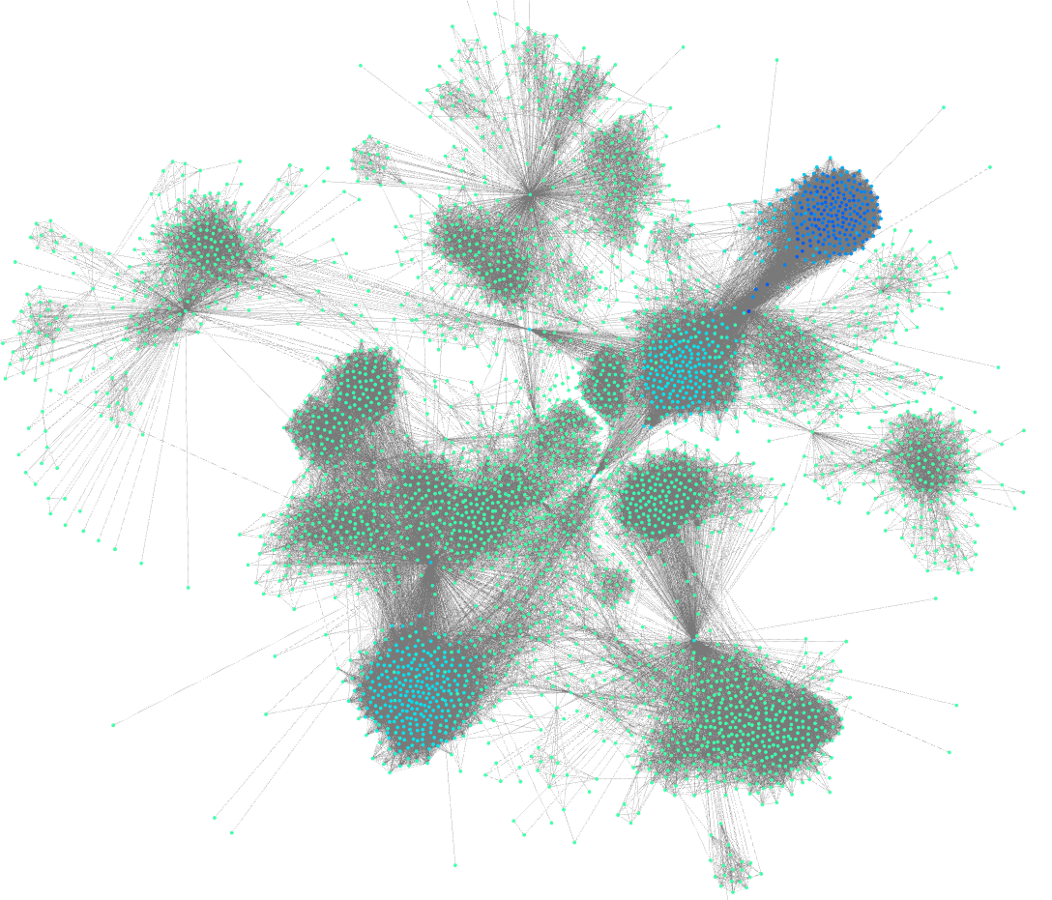
\includegraphics[width=0.3\linewidth]{graphs/overview.PNG}
	}
	\centering
	\subfigure[Citeseer]{
		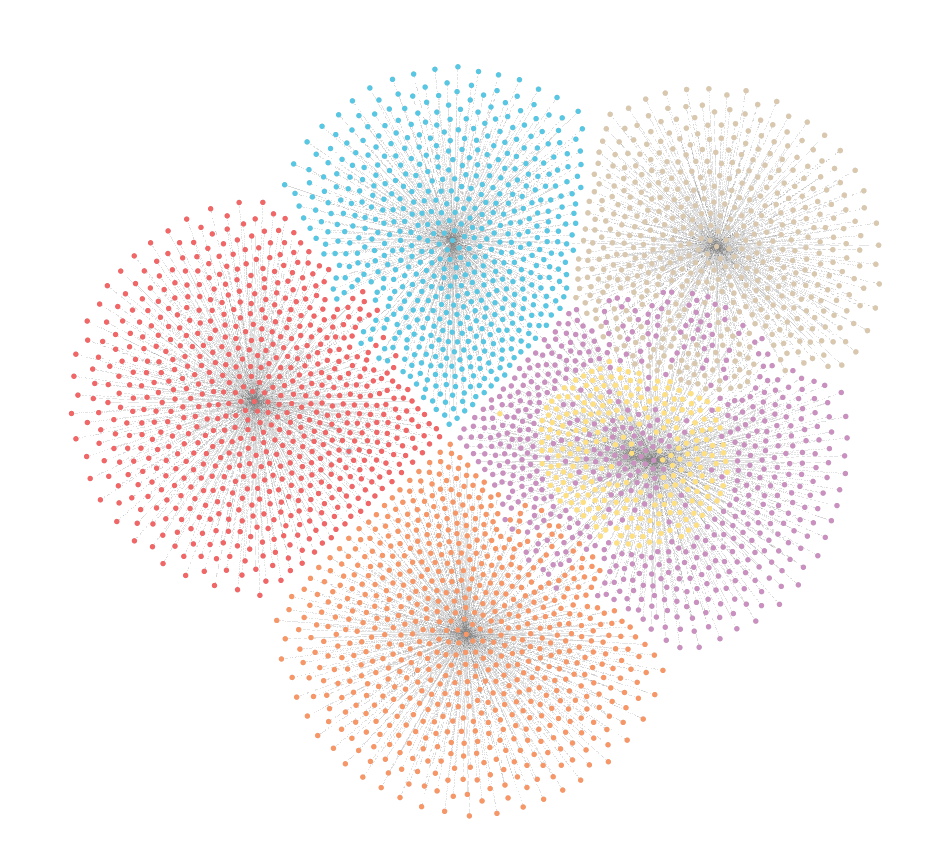
\includegraphics[width=0.25\linewidth]{citeseer/louvain.PNG}
	}
	\caption{Dataset Overview (powered by Neo4j)}
\end{figure}
The former dataset consists of 'circles' (or 'friends lists') from Facebook. It was collected from survey participants using this Facebook app. And the latter dataset consists of 3312 scientific publications classified into one of six classes. It includes publications described by a 0/1-valued word vector indicating the absence/presence of the corresponding word from the dictionary, which consists of 3703 unique words. The citation network consists of 4732 links. Here are the basic statistics and visualizations over the two datasets.
\begin{figure}[H]
	\centering
	\parbox{.4\linewidth}{
		\centering
		\begin{tabular} {cc}
			\hline\multicolumn{2}{c}{Ego-Facebook}\\
			\hline Nodes & 4039\\
			Edges & 88234\\
			Number of triangles & 1612010 \\
			Fraction of closed triangles & 0.2647\\
			Diameter (longest shortest path) & 8\\
			Average cost & 3.6925\\
		\end{tabular}
	}
\qquad\qquad
	\parbox{.4\linewidth}{
	\centering
	\begin{tabular} {cc}
		\hline\multicolumn{2}{c}{Citeseer}\\
		\hline Nodes & 3312\\
		Edges & 4732\\
		Number of triangles & 0 \\
		Fraction of closed triangles & 0\\
		Diameter (longest shortest path) & 6\\
		Average cost & 3.6541\\
	\end{tabular}
}
\caption{Network Data Statistics}
\end{figure}
\section{Degree, Centrality and Graph Analytics}
In this section, we will generally use ego-Facebook dataset for analytics.
\subsection{Zipf's Law}
Zipf's law is an empirical law that for many types of data studied in the physical and social sciences, the rank-frequency distribution exhibits an inverse relation, which belongs to a family of related discrete power law probability distributions. In most network data, the degree of each node also follows a certain power law, that is, $f(x)=ax^{-k}$. This is also true if we apply this natural rule to ego-Facebook network, because the following log-log has shown the property.
\begin{figure}[H]
	\centering
	\parbox{.45\linewidth}{
		\centering
		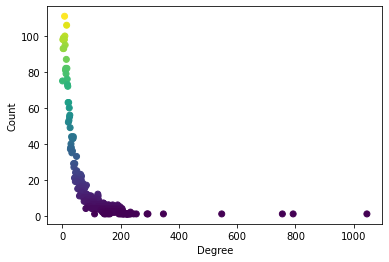
\includegraphics[width=.5\linewidth]{graphs/zipf's law1.PNG}
		\caption{Zipf's Law}
	}
	\parbox{.45\linewidth}{
	\centering
	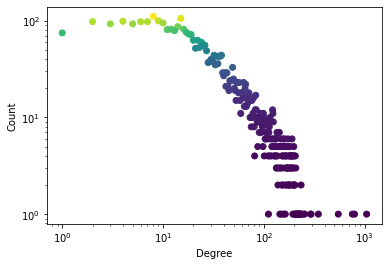
\includegraphics[width=.5\linewidth]{graphs/zipf's law.PNG}
	\caption{Zipf's Law (Under log-log)}
}
	\centering
\end{figure}
\subsection{Centrality Measures}
In graph theory and network analysis, indicators of centrality assign numbers or rankings to nodes within a graph corresponding to their network position. There are several different types of measures on node centrality described in the textbook\footnote{Zafarani, R. (2014). Social Media Mining: An Introduction (1st ed.). Cambridge University Press.} listed as follows,
\begin{figure}[H]
	\centering
	\parbox{.45\linewidth}{
		\centering
	\begin{tabular}{cc}
		\hline\multicolumn{2}{c}{Centrality}\\\hline
		Eigenvector & $c_v=\dfrac{1}{\lambda}\sum_{u\in N}c_u$\\
		PageRank & $C_p(v)=\alpha\sum_{j=1}A_{j,i}\dfrac{C_p(v_j)}{d_j^{out}}+\beta$\\
		Betweenness & $c_v=\sum_{s\ne v\ne t}\dfrac{\sigma_{s,t}(v)}{\sigma_{s,t}}$\\
		Closeness & $c_v=\dfrac{n-1}{\sum_{i\ne j}l_{i,j}}$	
	\end{tabular}
\caption{Table}
}
	\parbox{.45\linewidth}{
		\centering
	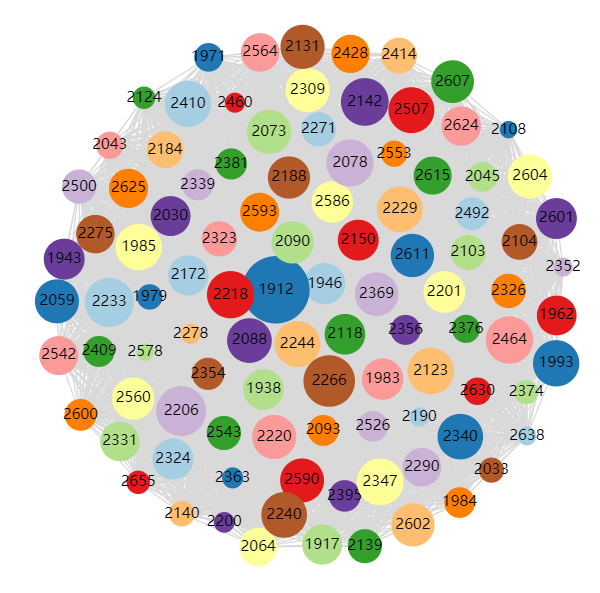
\includegraphics[width=0.5\linewidth]{graphs/eigenvector centrality.PNG}
\caption{Eigenvector Centrality}	
}
\end{figure}
We will only list top 5 nodes with respect to each centrality properties in order to get a clear overview of the difference between measures.
\begin{table}[H]
	\centering
	\parbox{.2\linewidth}{
		\centering
	\begin{tabular}{cc}
		\hline ID & Eigenvector\\\hline
		1912 & 296.5844\\
		2266 & 254.0166\\
		2206 & 250.4103\\
		2233 & 248.8579\\
		2142 & 245.7742
	\end{tabular}
}\quad
	\parbox{.2\linewidth}{
	\centering
	\begin{tabular}{cc}
		\hline ID & PageRank\\\hline
		3437 & 29.680\\
		107 & 27.084\\
		1684 & 24.785\\
		0 & 24.498\\
		1912 & 15.061
	\end{tabular}
}\quad
	\parbox{.2\linewidth}{
	\centering
	\begin{tabular}{cc}
		\hline ID & Betweenness\\\hline
		107 & 3916560\\
		1684 & 2753587\\
		3437 & 1924506\\
		1912 & 1868918\\
		1085 & 1214578
	\end{tabular}
}\quad
	\parbox{.2\linewidth}{
	\centering
	\begin{tabular}{cc}
		\hline ID & Closeness\\\hline
		107 & 0.4597\\
		58 & 0.3974\\
		428 & 0.3948\\
		563 & 0.3939\\
		1684 & 0.3936
	\end{tabular}
}
\caption{Difference}
\end{table}
As we can see from Table 1, Eigenvector Centrality cannot capture the essense of the topological structure of the network because all the nodes with high Eigenvector rankings gather in small clique. With iteration going on, all the centrality weights stream into several closely-related neighbour nodes, making them outrageously too powerful.
\section{Community Detection and Louvain Algorithm}
Community detection, also called graph partition, helps us to reveal the hidden relations among the nodes in the network. It can be used in machine learning to detect groups with similar properties and extract groups for various reasons. In our project, we aim to apply a famous Louvain method on ego-Facebook dataset, which was created by Blondel from the University of Louvain.\footnote{Blondel, Vincent D; Guillaume, Jean-Loup. "Fast unfolding of communities in large networks". Journal of Statistical Mechanics: Theory and Experiment. 2008 (10): P10008.}

\begin{definition}
	Communities refer to sets of tightly connected nodes.
\end{definition}
\begin{definition}
	Modularity $Q$ is a measure of how well a network is partitioned into communities estimated by the difference between the number of actual and expected edges within group $s$ expected. 
	\begin{align*}
		Q=\frac{1}{2m}\sum_{i,j}[A_{i,j}-\frac{k_ik_j}{2m}]\cdot\delta(c_i,c_j)
	\end{align*}
\end{definition}
The following Lemma will not have a exact proof, but it does play a key role in the acceleration of optimization process.
\begin{lemma}
	Modularity can be optimized by allowing only local changes to node-communities membership
	\begin{align*}
		\Delta Q(D \shortrightarrow i \shortrightarrow C) = \Delta Q(D \shortrightarrow i) + \Delta Q(i \shortrightarrow C)
	\end{align*}
\end{lemma}
And with this Lemma we can separate the Louvain algorithm into two phases.
\begin{algorithm}[H]
	\caption{Jenkins-Traub}
	\begin{algorithmic}
		\State\textbf{Phase 1:} Optimize Modularity allowing only local changes.
		\State$C = \argmax(\Delta D(D \shortrightarrow i \shortrightarrow C))$
		\State$D \shortleftarrow D - {i}$
		\State$C \shortleftarrow C + {i}$
		\State\textbf{Phase 2:} Aggregated small communities into super-nodes to build a new network.
		\State\textbf{Goto: Phase 1}
	\end{algorithmic}
\end{algorithm}

With the help of Neo4j, we can visualize the result as follows,
\begin{figure}[H]
	\centering
	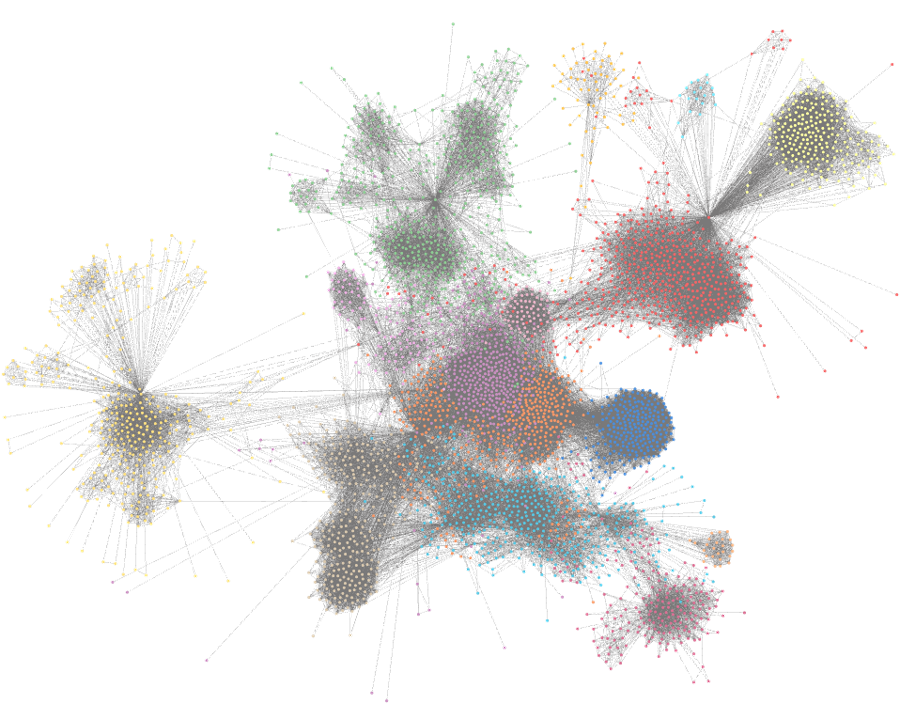
\includegraphics[width=.25\linewidth]{graphs/louvain2.PNG}
	\caption{Community Detection by Louvain Algorithm (Powered by Neo4j)}
\end{figure}
%-------------------------------------
\section{Link Prediction}
In network theory, link prediction is the problem of predicting the existence of a link between two entities in a network. This part we analysis Citeseer dataset with two methods: our Naïve Predictor and Graph InfoClust.
\subsection{Naïve Predictor}
We will select edge features like Common Neighbors, Jaccard's Coefficient, Adamic-Adar, Resource Allocation and Preferential Attachment discussed in the course listed as follows.

\begin{table}[H]
	\centering
	\begin{tabular}{cc}
		\hline\multicolumn{2}{c}{Similarity}                                                           \\\hline
		Common Neighbors        & $\Gamma(x)\cap\Gamma(y)$                                             \\
		Adamic-Adar             & $\Sigma_{Z\in \Gamma(x)\cap\Gamma(y)}\dfrac{1}{\log{| \Gamma(z) |}}$ \\
		Jaccard Coefficient     & $\dfrac{\Gamma(x)\cap\Gamma(y)}{\Gamma(x)\cup\Gamma(y)}$             \\
		Resource Allocation     & $\Sigma_{Z\in \Gamma(x)\cap\Gamma(y)}\dfrac{1}{| \Gamma(z) |}$       \\
		Preferential Attachment & $|\Gamma(x)| \cdot |\Gamma(y)|$
	\end{tabular}
	\caption{Features}
\end{table}

Since our naïve predictor doesn't have a good speed-up for large-scale data preprocessing, we have to shift our focus from the whole ego-Facebook network to a tailored subgraph, which contains 8823 positive edges and 8823 negative edges randomly picked from the original network. 75\% will be used as training set and the rest will be used as test set. The results with different choices on classifier are as follows:
\begin{figure}[H]
	\centering
	\parbox{.45\linewidth}{
		\centering
		\begin{tabular}{cc}
			\hline Classifier & Accuracy \\\hline
			SVM               & 67.9\%   \\
			Logistic          & 66.5\%   \\
			MLP               & 68.1\%
		\end{tabular}
	\caption{Naïve Predictor results}
	}
	\parbox{.45\linewidth}{
			\centering
		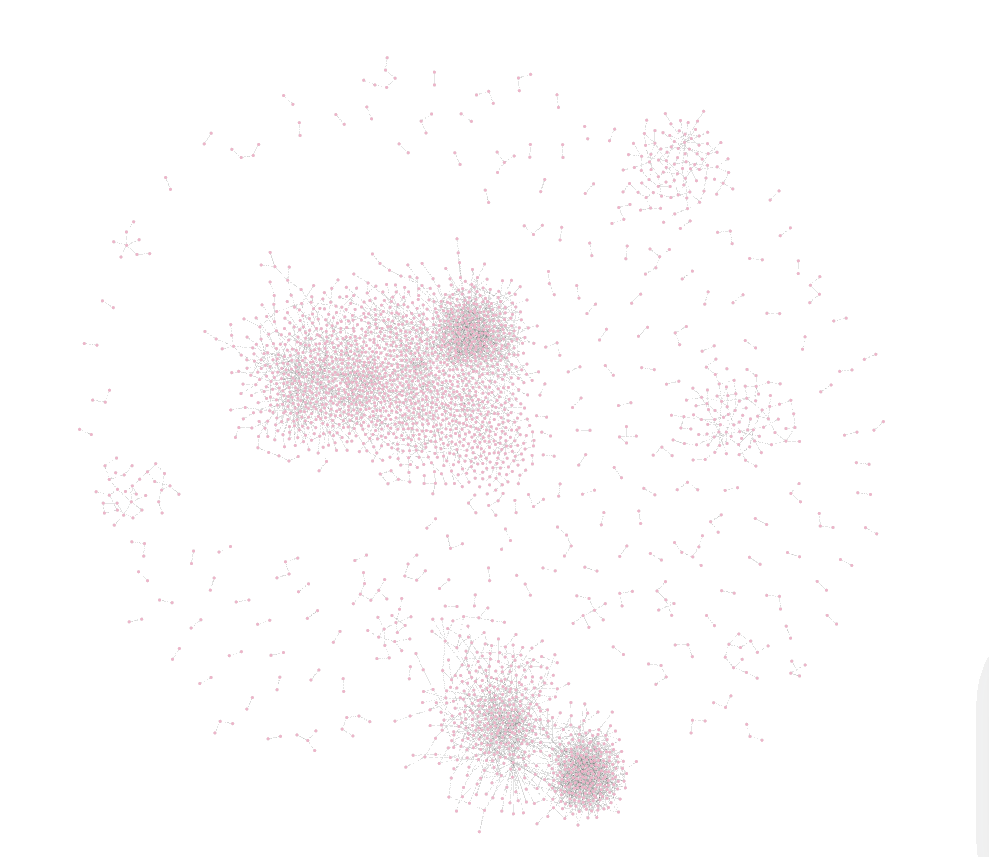
\includegraphics[width=.3\linewidth]{graphs/subgraph.PNG}
		\caption{Subgraph}
	}
\end{figure}
\subsection{Graph InfoClust (GIC)\footnote{Costas Mavromatis, George Karypis, Graph InfoClust: Leveraging cluster-level node information for unsupervised graph representation learning, PAKDD 21}}
In most graphs,there is significantly more structure that can be captured, e.g., nodes tend to belong to (multiple) clusters that represent structurally similar nodes. Motivated by this observation, we propose a graph representation learning method called Graph InfoClust (GIC), that seeks to additionally capture cluster-level information content. These clusters are computed by a differentiable K-means method and are jointly optimized by maximizing the mutual information between nodes of the same clusters. This optimization leads the node representations to capture richer information and nodal interactions, which improves their quality.

Graph InfoClust relies on a framework similar to DGI’s to optimize the embedding space so that it contains additional cluster-level information content. The novel idea is to learn node representations by maximizing the mutual information between (i) node (fine-grain) representations and the global graph summary, and (ii) node (fine-grain) representations and corresponding cluster (coarse-grain) summaries. This enables the embeddings to be mindful of various structural properties and avoids the pitfall of optimizing the embeddings based on a single vector.

In clustering, the goal is to cluster together related nodes (e.g., nodes that belong to the same class) without any label information. The computed embeddings are clustered into K = \#classes clusters with K-means. The evaluation is provided by external labels, the same used for node classification.

In link prediction, some edges are hidden in the input graph and the goal is to predict the existence of these edges based on the computed embeddings. We follow the setup: 5\% of edges and negative edges as validation set, 10\% of edges and negative edges as test set, F0 = 16, and the results are averaged over 10 runs. We report the area under the ROC curve (AUC) score, which is equal to the probability that a randomly chosen edge is ranked higher than a randomly chosen negative edge, and the average precision (AP) score, which is the area under the precision-recall curve; here, precision is given by TP/(TP+FP) and recall by TP/(TP+FN).

Setting parameters $\alpha,\beta,K=0.5,100,128$, we got results like: AUC = 97\%, AP = 97\%, better than the prediction given by Naïve Predictor.

\section{Node Classification Task on Graph Data}

In this section we focus on the task of node classification. We will mainly introduce four models which achieved excellent performance in node classification in recent years, and we think these models can be regarded as cutting-edge methods in the task of graph data structure node classification, and these models can reflect the development trend and achievement of node classification tasks in recent years.

\subsection{GIC\footnote{Costas Mavromatis, George Karypis. Graph InfoClust: Leveraging cluster-level node information for unsupervised graph representation learning. PAKDD 2021.}}

The goal is to predict some (or all) of the nodes’ labels based on a given (small) training set. In unsupervised methods, the learned node embeddings are passed to a downstream classifier, e.g., logistic regression. Following, we sample 20$\times$classes nodes as the train set, $30\times\texttt{\#}$ classes nodes as the validation set, and the remaining nodes are the test set. The sets are either uniformly drawn from each class (balanced sets) or randomly sampled (imbalanced sets). For the unsupervised methods, we use a logistic regression classifier, which is trained with a learning rate of 0.01 for 1k epochs with Adam SGD optimizer and Glorot initialization. The classification accuracy (Acc) is reported as a performance metric, which is the percentage of correctly classified instances (TP + TN)/(TP + TN + FP + FN) where TP, FN, FP, and TN represent the number of true positives, false negatives, false positives, and true negatives, respectively.
\begin{figure}[H]
	\centering
	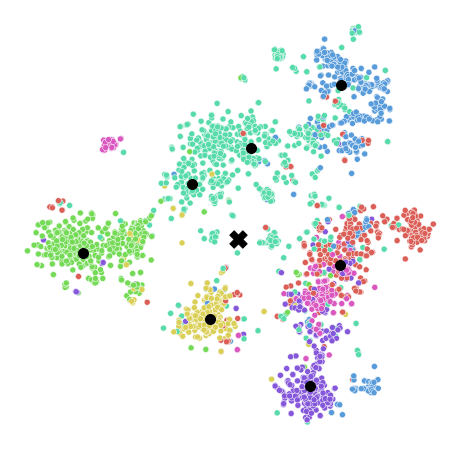
\includegraphics[width=.25\linewidth]{graphs/GIC.PNG}
	\caption{Node Classification}
\end{figure}

\subsection{Kernel GCN\footnote{Yu Tian, Long Zhao, Xi Peng, Dimitris N. Metaxas. Rethinking Kernel Methods for Node Representation Learning on Graphs. NeurIPS 2019.}}

Graph Kernel\footnote{N. M. Kriege, M. Neumann, C. Morris, K. Kersting, and P. Mutzel. A unifying view of explicit and implicit feature maps for structured data: systematic studies of graph kernels. arXiv preprint arXiv:1703.00676, 2017.} is a classic method for graph classification tasks\footnote{M. Draief, K. Kutzkov, K. Scaman, and M. Vojnovic. KONG: Kernels for ordered-neighborhood graphs. In Advances in Neural Information Processing Systems (NeurIPS), pages 4051–4060, 2018.}\footnote{T. N. Kipf and M. Welling. Semi-supervised classification with graph convolutional networks.In Proceedings of the International Conference on Learning Representations (ICLR), 2017.}   based on the kernel method, but it is not suitable for more fine-grained node classification tasks\footnote{S. Abu-El-Haija, A. Kapoor, B. Perozzi, and J. Lee. N-GCN: Multi-scale graph convolution for semi-supervised node classification. arXiv preprint arXiv:1802.08888, 2018.}\footnote{L. Zhang, H. Song, and H. Lu. Graph node-feature convolution for representation learning.
	arXiv preprint arXiv:1812.00086, 2018.}; the former is related to the representation learning of the entire graph, and the latter corresponds to the node representation learning. And the cutting-edge results of this method rely on manual selection of heuristic functions. Inspired by the kernel-based-method in the graph classification task, and further capture the graph structure information, the KernelGCN method provides a transition between the above two tasks. In theory, it can be proved that Kernel GCN can realize any positive semi-definite kernel, thus ensuring its expressive ability. At the same time, the algorithm designs an efficient similarity measurement and feature aggregation process to accelerate training.

\subsection{GCNII\footnote{Ming Chen, Zhewei Wei, Zengfeng Huang, Bolin Ding, Yaliang Li. Simple and Deep Graph Convolutional Networks. ICML 2020.
}} 

GCNII is a deep learning method on graph-related problems based on GCN\footnote{Thomas N. Kipf, Max Welling. Semi-Supervised Classification with Graph Convolutional Networks. ICLR 2017.} . Although GCN can capture graph structure information and feature information on graph-related issues, it faces an over-smoothing\footnote{Chen Cai, Yusu Wang. A Note on Over-Smoothing for Graph Neural Networks. ICML 2020 Graph Representation Learning workshop. }  problem: as the network depth increases, the representation of each node tends to be consistent. The over-smoothing problem limits the depth of the GCN model. ResNet\footnote{Kaiming He, Xiangyu Zhang, Shaoqing Ren, Jian Sun. Deep Residual Learning for Image Recognition.}  uses the residual connections design to solve the network depth problem in the non-graph field, but the SOTA model based on GCN, GAT\footnote{Petar Veličković, Guillem Cucurull, Arantxa Casanova, Adriana Romero, Pietro Liò, Yoshua Bengio. Graph Attention Networks. ICLR 2018.} , etc., in the related tasks on the graph network is still a two-layer network structure. JKNet\footnote{Keyulu Xu, Chengtao Li, Yonglong Tian, Tomohiro Sonobe, Ken-ichi Kawarabayashi, Stefanie Jegelka. Representation Learning on Graphs with Jumping Knowledge Networks. ICML 2018.}  and DropEdge\footnote{Yu Rong, Wenbing Huang, Tingyang Xu, Junzhou Huang. DropEdge: Towards Deep Graph Convolutional Networks on Node Classification.}  models have made many attempts on over-smoothing problems, but the results are not ideal: experiments show that these models only slow down the performance degradation caused by the increase of network depth, but do not solve this problem. The performance of shallow models Still have to exceed the deep model. On the other hand, models such as SGC \footnote{Felix Wu, Tianyi Zhang, Amauri Holanda de Souza Jr., Christopher Fifty, Tao Yu, Kilian Q. Weinberger. Simplifying Graph Convolutional Networks. ICML 2019. } and PPNP \footnote{Johannes Klicpera, Aleksandar Bojchevski, Stephan Günnemann. Predict then Propagate: Graph Neural Networks meet Personalized PageRank. ICLR 2019.} try to solve the over-smoothing problem faced by traditional deep models by combining shallow models and propagation algorithms. However, these models perform linear combinations of neighbor node features at each layer, which is essentially shallow. Models do not have the powerful expressive ability of in-depth models. GCNII adds two structures: Initial residual and Identity mapping, which solves the over-smoothing problem in deep networks; and the following theoretical analysis compares the difference between GCN and GCNII to prove its effectiveness.

\subsection{SSP\footnote{Mohammad Rasool Izadi, Yihao Fang, Robert Stevenson, Lizhen Lin. Optimization of Graph Neural Networks with Natural Gradient Descent. https://arxiv.org/abs/2008.09624}} 

The optimization step of SSP in deep network training has improved it. It uses natural gradients instead of traditional gradients in graph-based semi-supervised learning tasks, making model training and inference processes more efficient. Experiments have proved that the training efficiency of the model using this optimization method exceeds that of the traditional optimization methods such as ADAM\footnote{Diederik P. Kingma, Jimmy Ba. Adam: A Method for Stochastic Optimization. 3rd International Conference for Learning Representations, San Diego, 2015.}  and SGD\footnote{Sebastian Ruder. An overview of gradient descent optimization algorithms. https://arxiv.org/abs/1609.04747} .

Finally, let's compare the Accuracy results of the above three methods on the Cora  data set:
\begin{table}[H]
	\centering	
	\parbox{.4\linewidth}{
		\centering
	\begin{tabular}{cc}
		\hline\multicolumn{2}{c}{Accuracy}\\
		\hline
		GIC & 0.7317\\
		Kernel GCN & 0.8010\\
		GCNII & 0.8540\\
		SSP & 0.8709
	\end{tabular}
}
	\parbox{.55\linewidth}{
		\centering
		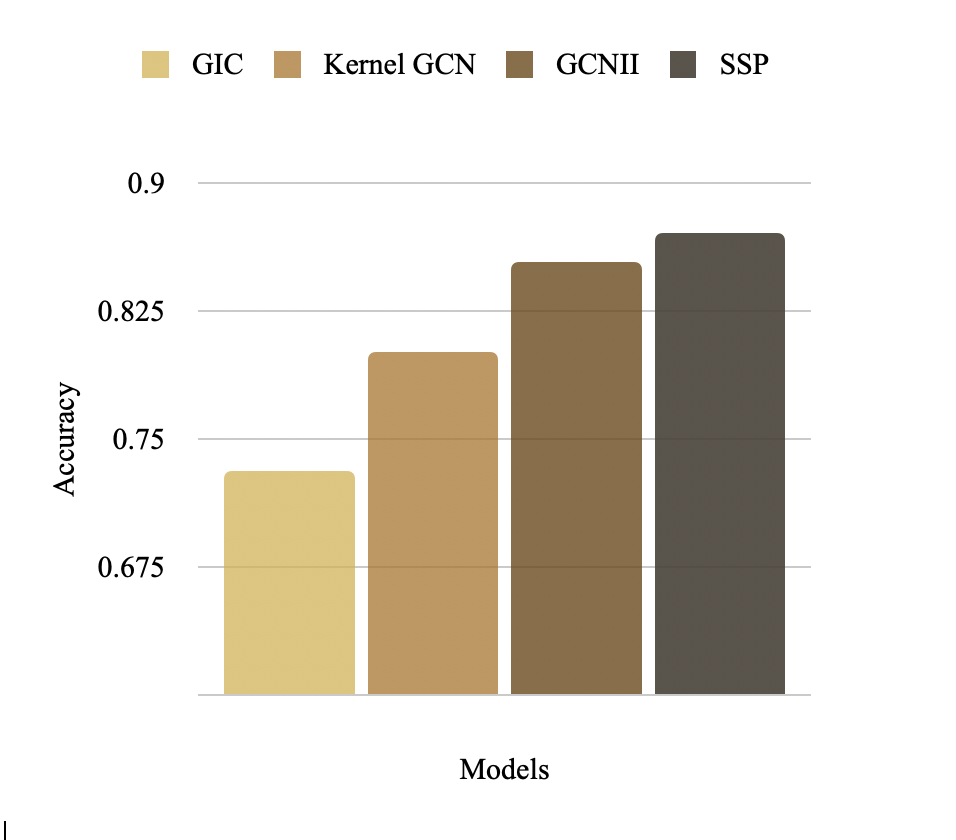
\includegraphics[width=.5\linewidth]{graphs/Comparison.PNG}
	}	
	
	\caption{Accuracy of Different Models on Cora Data set}
	
\end{table}
%=====================
\end{document}
